\documentclass{standalone}
\usepackage{pgfplots}
\pgfplotsset{compat=1.17}
\usetikzlibrary{arrows.meta}

\begin{document}

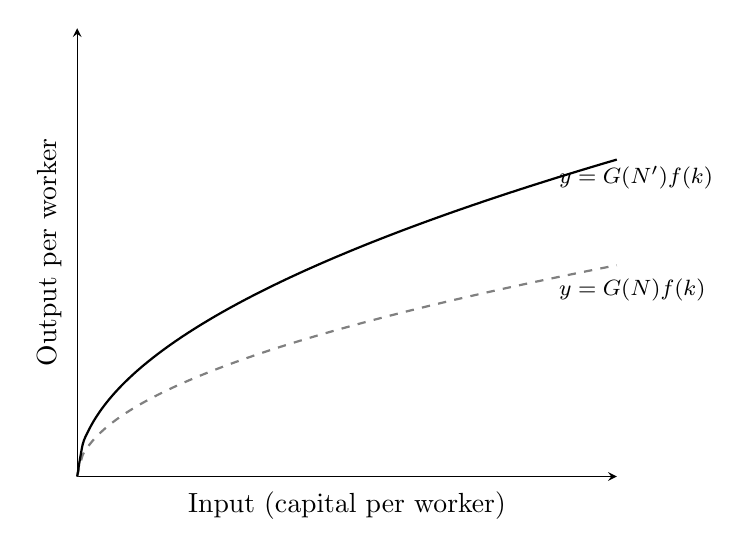
\begin{tikzpicture}
    \begin{axis}[
        axis lines=left,
        xmin=0, xmax=8,
        ymin=0, ymax=6,
        xlabel={Input (capital per worker)},
        ylabel={Output per worker},
        xtick=\empty,
        ytick=\empty,
        enlargelimits=false,
        clip=false,
        domain=0:8,
        samples=100,
        every axis plot post/.append style={
            thick,
            smooth
        }
    ]
        
        % Production function for N
        \addplot [gray, dashed] {x^0.5};
        \node [right, font=\footnotesize] at (axis cs:7, 2.5) {$y = G(N)f(k)$};
        
        % Production function for N'
        \addplot [black] {1.5*x^0.5};
        \node [right, font=\footnotesize] at (axis cs:7, 4.0) {$y = G(N')f(k)$};
        
    \end{axis}
\end{tikzpicture}

\end{document}